%! Tex program = pdflatex
 
\documentclass[UTF8]{ctexart}
\CTEXsetup[format={\Large\bfseries}]{section}
\usepackage{amsmath}
\usepackage{ctex}
\usepackage{array}
\usepackage{ulem}
\usepackage{graphicx}
\usepackage{geometry}
\usepackage{multirow}
\usepackage{subfig}
\usepackage{float}
\usepackage{multicol}
\usepackage{multirow}
\usepackage{indentfirst}
\usepackage{makecell}
\geometry{papersize={21cm,29.7cm}}
\geometry{left=2.54cm,right=2.54cm,top=3.18cm,bottom=3.18cm}
\usepackage{fancyhdr}
\pagestyle{fancy}
\lhead{\today}
\chead{}
\rhead{2020011075}
\lfoot{清华大学}
\cfoot{\thepage}
\rfoot{系统工程导论}
\renewcommand{\headrulewidth}{0.4pt}
\renewcommand{\headwidth}{\textwidth}
\renewcommand{\footrulewidth}{0pt}
\usepackage{bm}

\begin{document}

\begin{center}
  \textbf{\LARGE{系统工程导论作业三——黑箱建模1}}\\
\end{center}
\begin{center}
  \large{彭程 2020011075}
\end{center}
\section{题目一}

\subsection{回归直线方程}
根据一元线性回归方程计算公式:

$$
b = \frac{\sum (x_{i}-\overline{x})(y_{i}-\overline{y})}{\sum (x_{i}-\overline{x})^{2}}$$
 
$$
a = \overline{y}-b\overline{x}
$$

利用python编程代入数据计算可得到:
$$
b=0.346467
$$
$$
a=2129616.766806
$$

\subsection{F检验法进行统计检验}
由F检验法,一元线性回归时有:
$$
F=\frac{E S S / f_{E}}{R S S / f_{R}}=\frac{(N-2) E S S}{R S S}
$$


对于给定的显著性水平$\alpha(0 \leq \alpha \leq 1)$,以及自由度 (1,N-2),查F分布表,得到相应的临界值$F_\alpha$,从而对$H_0$进行假设检验,有:

当F >$F_\alpha$时,否定原假设,认为 x 与 y 存在线性关系;

当F ≤ $F_\alpha$时,接收原假设,认为 x 与 y 不存在线性关系。

程序计算结果为:

$$
F = 663.411691 > F_\alpha = 4.351244
$$

即说明x与y存在线性关系


\subsection{置信区间}

给定显著性水平  $\alpha$  ,对某一  $\mathrm{x}_{0}$  ,相应的 $ \mathrm{y}_{0}$  将以  $(1-\alpha) $ 的概率落在置信区间:
$$
\left(\hat{y}_{0}-Z_{\alpha / 2} S_{\delta}, \hat{y}_{0}+Z_{\alpha / 2} S_{\delta}\right)
$$

其中$Z_{\alpha / 2}$  是标准正态分 布上  $\alpha / 2$  百分位点的值,
剩余均方差$S_{\sigma}=\sqrt{\frac{\sum_{i=1}^{N}\left(y_{i}-\hat{y}\right)^{2}}{N-2}}$

将数据代入公式计算得到置信区间为:
$$
(y - 180345.485494, y + 180345.485494)
$$

\subsection{程序运行结果}
\begin{figure}[H]
  \centering
  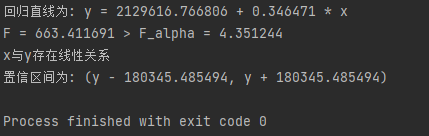
\includegraphics[scale=1.5]{result.png}
\end{figure}

\subsection{绘图}
在一个 figure 中, 绘出: a.数据点, b.回归直线, c.置信区间相应的两条边界直线。

置信区间边界直线:
$$
\begin{array}{l}
L_{1}: y_{1}=a+b x-Z_{\alpha / 2} S_{\delta} \\
L_{2}: y_{1}=a+b x+Z_{\alpha / 2} S_{\delta}
\end{array}
$$

图像如下:

\begin{figure}[H]
  \centering
  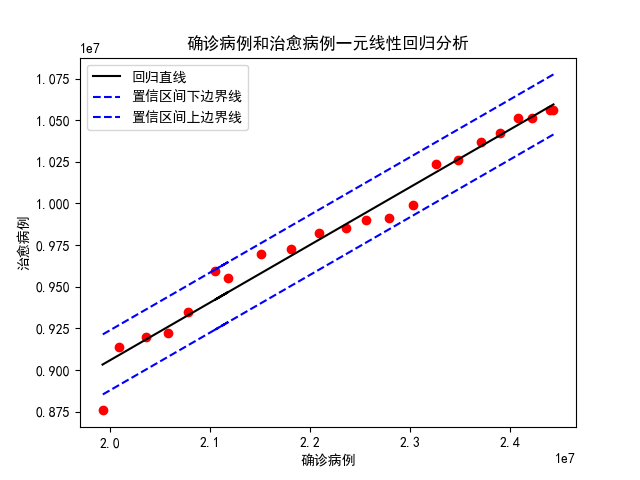
\includegraphics[scale=0.8]{回归分析.png}
\end{figure}



\end{document}